\lfoot{Autor: Fitim Faiku}
\subsubsection{Kompatible Geräte}
\label{subsec:device-compability}

Android kann auf vielen verschiedenen Plattformen, wie Handys oder Tabletts laufen.
Als Entwickler bietet die Palette von Geräten ein enormes potenzielles Publikum.
Um auf all diesen Oberflächen reibungslos zu funktionieren muss eine App einige Feature Variabilitäten tolerieren und eine 
flexible Benutzeroberfläche zur Verfügung stellen. 

Um das zu ermöglichen bietet Android die Möglichkeit, verschiedene XML Layouts zu erstellen um verschiedene Bildschirmgrößen anzusprechen.

Beim Programmieren der App kann auch die minimale und maximale kompatible Android-Version des Devices eingestellt werden, wobei hier eine möglichst umfangreiche Auswahl der Versionen einen größeren Umfang an Nutzern erzielt.

\begin{figure}[!htb]\centering
	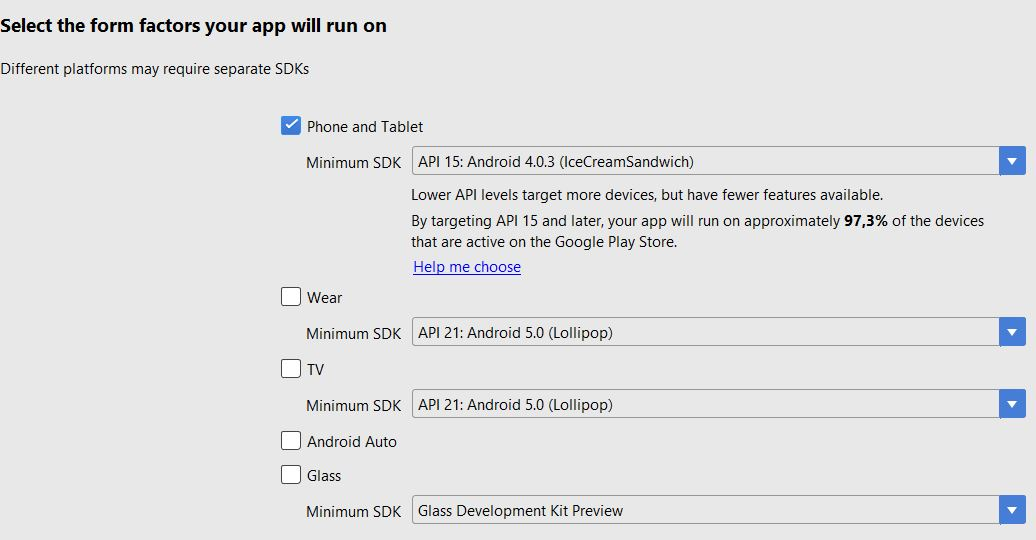
\includegraphics[width=1.0 \textwidth]{images/MinMaxVers}
	\caption{Version}\label{Fig:min-max Version}
\end{figure}



\clearpage % DO NOT REMOVE